%++++++++++++++++++++++++++++++++++++++++
% Don't modify this section unless you know what you're doing!
\documentclass[letterpaper,12pt]{article}
\usepackage{tabularx} % extra features for tabular environment
\usepackage{amsmath}  % improve math presentation
\usepackage{graphicx} % takes care of graphic including machinery
\usepackage[margin=1in,letterpaper]{geometry} % decreases margins
\usepackage[final]{hyperref} % adds hyper links inside the generated pdf file
\hypersetup{
	colorlinks=true,       % false: boxed links; true: colored links
	linkcolor=blue,        % color of internal links
	citecolor=blue,        % color of links to bibliography
	filecolor=magenta,     % color of file links
	urlcolor=blue         
}
%++++++++++++++++++++++++++++++++++++++++

\usepackage{titling}
\pretitle{\begin{flushright}}
\posttitle{\par\end{flushright}}
\preauthor{\begin{flushright}}
\postauthor{\par\end{flushright}}
\predate{\begin{flushright}}
\postdate{\par\end{flushright}}

\usepackage[font=small,skip=0pt]{caption}

% \usepackage[demo]{graphicx}
\usepackage{subcaption}
\usepackage{float}

\usepackage{booktabs}

\usepackage[style=ieee,backend=biber]{biblatex}
\addbibresource{report.bib}

\begin{document}

\title{\vspace{-2cm} Kavi Dey}
\author{\vspace{-0.4cm} E157 RF Design \\ Lab Partner: Zoe Worrall \\ Design Project 2}
\date{\vspace{-0.4cm} \today}
\maketitle

% modified from https://www.overleaf.com/latex/templates/sample-lab-report-for-u-of-r-phys-349/pgsyqngcyjxk
%++++++++++++++++++++++++++++++++++++++++

% abstract
% \begin{abstract}
% abstract here
% \end{abstract}

% sections
\section{Summary Information}
The secret message is ``HMC''. The maximum range that we predicted our receiver would work at was XX m.
The maximum range we were able to test was 72.3 m due to running out of cable length in the hallway.
The analytical system temperature was 8.22E+10 K and the measured temperature was 7.13E+07 K.
The analytical receiver IIP3 was 7.53 dBm and the measured one was XX dBm.

\newpage
\section{Pictures of Received Data}
\begin{figure}[H]
	\begin{centering}
		\includegraphics[width=0.5\columnwidth,angle=-90]{figures/3m.img}
		\caption{Picture of setup at 3 m range}
	\end{centering}
\end{figure}

\begin{figure}[H]
	\begin{centering}
		\includegraphics[width=0.5\columnwidth]{figures/3m.trace}
		\caption{Oscilloscope trace at 3 m range}
	\end{centering}
\end{figure}

\begin{figure}[H]
	\begin{centering}
		\includegraphics[width=0.5\columnwidth]{figures/3m.spectra}
		\caption{Spectrum at 3 m range}
	\end{centering}
\end{figure}

\begin{figure}[H]
	\begin{centering}
		\includegraphics[width=0.5\columnwidth]{figures/maxm.img}
		\caption{Picture of setup at max range}
	\end{centering}
\end{figure}

\begin{figure}[H]
	\begin{centering}
		\includegraphics[width=0.5\columnwidth]{figures/maxm.trace}
		\caption{Oscilloscope trace at max range}
	\end{centering}
\end{figure}

\begin{figure}[H]
	\begin{centering}
		\includegraphics[width=0.5\columnwidth]{figures/maxm.spectra}
		\caption{Spectrum at max range}
	\end{centering}
\end{figure}


\newpage
\section{Oscilloscope Trace Decoding}
\begin{figure}[H]
	\begin{centering}
		\includegraphics[width=0.7\columnwidth]{example-image-a}
		\caption{Annotated oscilloscope trace for decoding}
	\end{centering}
\end{figure}

\newpage
\section{Antenna Information}
\begin{figure}[H]
	\begin{centering}
		\includegraphics[width=0.8\columnwidth]{figures/antenna}
		\caption{Hawking H-A16SD Antenna}
	\end{centering}
\end{figure}

\newpage
\section{Receiver Schematic}
\begin{figure}[H]
	\begin{centering}
		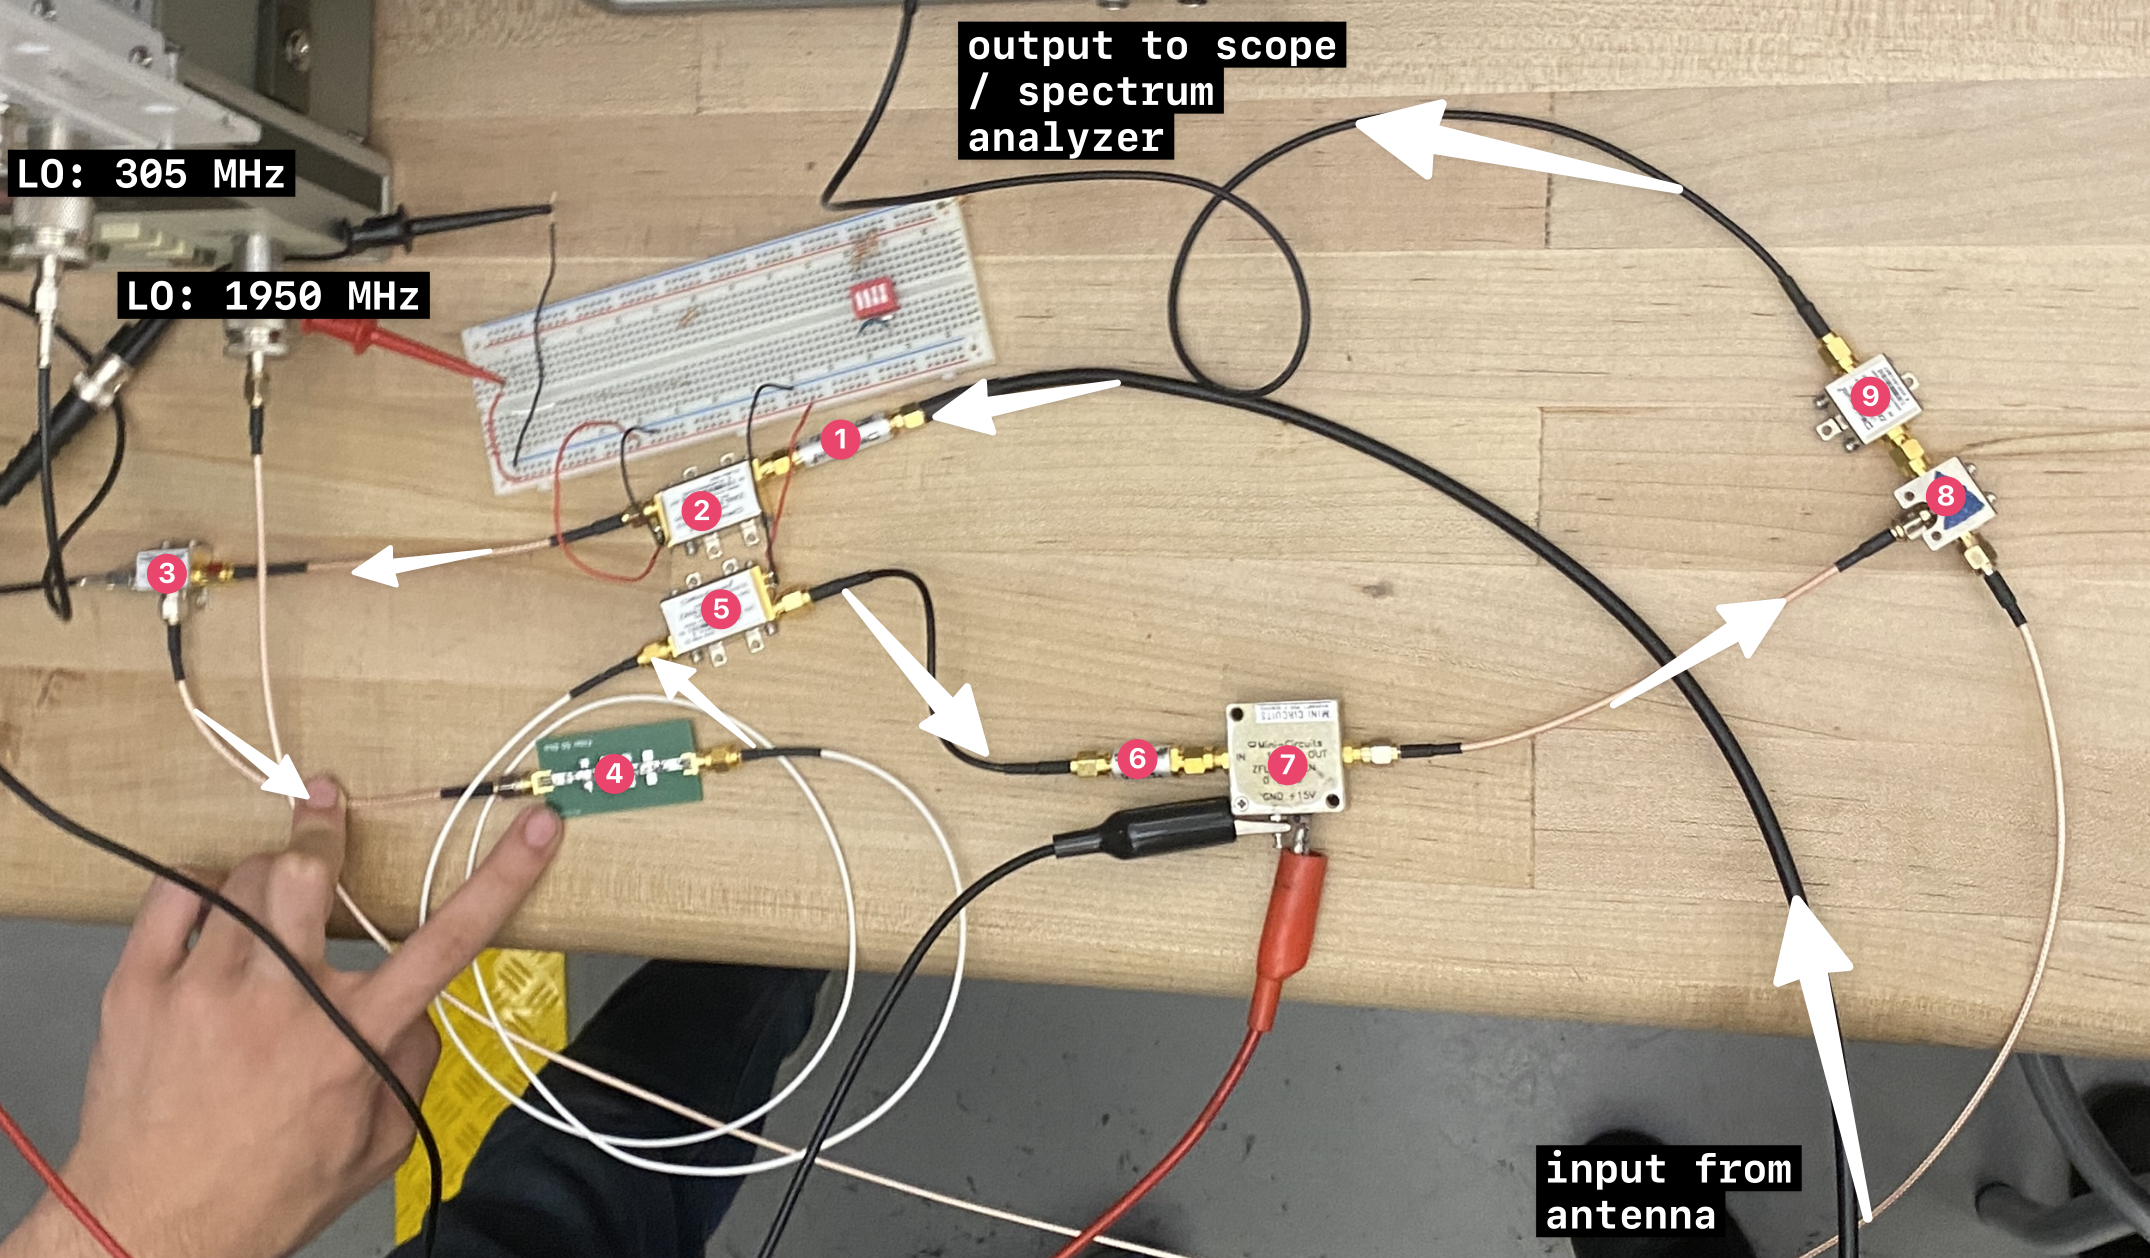
\includegraphics[width=1\columnwidth]{figures/receiver_picture.png}
		\caption{Picture of Receiver}
	\end{centering}
\end{figure}

\begin{figure}[H]
	\begin{centering}
		\includegraphics[width=1\columnwidth]{figures/receiver_schematic.pdf}
		\caption{Receiver Schematic}
	\end{centering}
\end{figure}

The custom bandpass filter was built as a 2nd order chebyshev filter designed using \href{https://markimicrowave.com/technical-resources/tools/lc-filter-design-tool/}{Marki LC Filter Design Tool}. The S21 log magnitude is provided below for reference
\begin{figure}[H]
	\begin{centering}
		\includegraphics[width=1\columnwidth]{figures/bpf_s21.png}
		\caption{Custom Bandpass filter S21}
	\end{centering}
\end{figure}

\newpage
\section{Receiver Spectra}
\begin{figure}[H]
	\begin{centering}
		\includegraphics[width=0.5\columnwidth]{figures/receiver_spectra/0.beginning}
		\caption{Stage 0: Raw antenna spectra}
	\end{centering}
\end{figure}

\begin{figure}[H]
	\begin{centering}
		\includegraphics[width=0.5\columnwidth]{figures/receiver_spectra/1.bpf}
		\caption{Stage 1: After wide bandpass filter}
	\end{centering}
\end{figure}

\begin{figure}[H]
	\begin{centering}
		\includegraphics[width=0.5\columnwidth]{figures/receiver_spectra/2.amp}
		\caption{Stage 2: After amplifier}
	\end{centering}
\end{figure}

\begin{figure}[H]
	\begin{subfigure}[t]{.49\textwidth}
		\centering
		\includegraphics[width=\linewidth]{figures/receiver_spectra/3.mixer.lower}
		\caption{IF Spectra}
	  \end{subfigure}
	  \hfill
	  \begin{subfigure}[t]{.49\textwidth}
		\centering
		\includegraphics[width=\linewidth]{figures/receiver_spectra/3.mixer.upper}
		\caption{RF Spectra}
	  \end{subfigure}

	  \vspace{0.5cm}
	  \caption{Stage 3: After mixer (LO = 1950 MHz)}
\end{figure}

\begin{figure}[H]
	\begin{centering}
		\includegraphics[width=0.5\columnwidth]{figures/receiver_spectra/4.bpf}
		\caption{Stage 4: After bandpass filter}
	\end{centering}
\end{figure}

\begin{figure}[H]
	\begin{centering}
		\includegraphics[width=0.5\columnwidth]{figures/receiver_spectra/5.amp}
		\caption{Stage 5: After amplifier}
	\end{centering}
\end{figure}

\begin{figure}[H]
	\begin{centering}
		\includegraphics[width=0.5\columnwidth]{figures/receiver_spectra/6.attenuator}
		\caption{Stage 6: After attenuator}
	\end{centering}
\end{figure}

\begin{figure}[H]
	\begin{centering}
		\includegraphics[width=0.5\columnwidth]{figures/receiver_spectra/7.amp}
		\caption{Stage 7: After amplifier}
	\end{centering}
\end{figure}

\begin{figure}[H]
	\begin{subfigure}[t]{.49\textwidth}
		\centering
		\includegraphics[width=\linewidth]{figures/receiver_spectra/8.mixer.lower}
		\caption{IF Spectra}
	  \end{subfigure}
	  \hfill
	  \begin{subfigure}[t]{.49\textwidth}
		\centering
		\includegraphics[width=\linewidth]{figures/receiver_spectra/8.mixer.upper}
		\caption{RF Spectra}
	  \end{subfigure}

	  \vspace{0.5cm}
	  \caption{Stage 8: After mixer}
\end{figure}

\begin{figure}[H]
	\begin{subfigure}[t]{.49\textwidth}
		\centering
		\includegraphics[width=\linewidth]{figures/receiver_spectra/9.lpf.lower}
		\caption{IF Spectra}
	  \end{subfigure}
	  \hfill
	  \begin{subfigure}[t]{.49\textwidth}
		\centering
		\includegraphics[width=\linewidth]{figures/receiver_spectra/9.lpf.upper}
		\caption{RF Spectra}
	  \end{subfigure}

	  \vspace{0.5cm}
	  \caption{Stage 9: After lowpass filter}
\end{figure}

\newpage
\section{Theoretical Signal and Noise Levels}

\newpage
\section{IP3 Distortion Characterization}
To measure the IIP3 of our amplifier we replaced the antenna with a two tone signal generator. We tested a range of input powers and measured the output power of the fundamental and the IM3 terms to make the following plot.
\begin{figure}[H]
	\begin{centering}
		\includegraphics[width=0.7\columnwidth]{figures/iip3_regression.pdf}
		\caption{Analytical and measured IIP3}
	\end{centering}
\end{figure}
Running a linear regression we get:
\\
\begin{center}
	\begin{tabular}{lrr}
		\toprule
		Term & Slope & Intercept \\
		\midrule
		Linear & 1.21 & 30.12 \\
		3rd Order & 2.9 & 75.34 \\
		\bottomrule
	\end{tabular}
\end{center}

\noindent
To calculate the analytical IP3 point we used the following logic. We only need to consider the IM3 components generated by the last amplifier because they are orders of magnitude larger than the earlier ones. This allows us to simplify the receiver chain into gain $\to$ amplifier $\to$ attenuation.
\\
\\
\noindent
Adding additional (assumed perfectly linear) gain $G$ before the final amplifier reduces the input power needed to achieve the same output power. In other words reduces $IIP3$ to $IIP3_{combined} = IIP3_{amplifier} - G$ while keeping the same $OIP3$. Adding additional attenuation $L$ after the final amplifier reduces the total output, keeping $IIP3$ the same and reducing $OIP3$ to $OIP3_{combined} = OIP3_{amplifier} - L$.
\\
\\
\noindent
Our final amplifier (stage 7) is the ZFL-1000LN which has an $IIP3$ of -6.4 dBm and $OIP3$ of 14 dBm. Adding up all the amplification and attenuation from stages 1-6, we get $G$ = 56.1 dBm and addding up the attenuation from stages 8-9 we get $L$ = -7 dBm. This results in analytical $IIP3$ = -62.5 and $OIP3$ = 7 dBm.

% Pout vs. Pin plot showing fundamental power and IM3 power at the output of your receiver in the receiver characterization test configuration.
% Extrapolate measured lines to indicate a measured IP3.
% Include a point showing your theoretical IP3.
% Include a calculation below (with references to datasheets where appropriate) to explain how you calculated your theoretical IP3.

% \newpage
% \section{Discussions \label{sec:discussion}}
% Discussion of discrepancies between analytical, simulated and measured results.  Quantitatively justify differences between them, including any modifications you made to your models to make your simulations match your measurements better (e.g.: board parasitics).  Refer to prior figures in your report for supporting evidence in this discussion.

\section{Additional Notes}
All of the data, code, and figures are available in this github repo: \url{github.com/kavidey/e157/tree/main/dp_02}.
\begin{enumerate}
  \item \texttt{schematics/} has the pretty display schematics made in Altium
\end{enumerate}

% \newpage
% \section{Takeaways}
% One paragraph about one thing you learned about RF design doing this project.

% \newpage
% \section{Bibliography}
% \printbibliography

% referencing bibliography
% ~\cite{melissinos, Cyr, Wiki}

% figures
% \begin{figure}[ht] 
%     \centering \includegraphics[width=0.8\columnwidth]{sr_setup}
%     \caption{
%             \label{fig:samplesetup}
%             Every figure MUST have a caption.
%     }
% \end{figure}

% equations
% \begin{equation} \label{eq:aperp} % the label is used to reference the equation
%     u(\lambda,T)=\frac{8\pi hc\lambda^{-5}}{e^{hc/\lambda kT}-1},
% \end{equation}
%
% ~\ref{fig:samplesetup}

% tables
% \begin{table}[ht]
%     \begin{center}
%         \caption{Every table needs a caption.}
%         \label{tbl:bins} % spaces are big no-no withing labels
%         \begin{tabular}{|cc|}
%             \hline
%             \multicolumn{1}{|c}{$x$ (m)} & \multicolumn{1}{c|}{$V$ (V)} \\
%             \hline
%             0.0044151                    & 0.0030871                    \\
%             0.0021633                    & 0.0021343                    \\
%             0.0003600                    & 0.0018642                    \\
%             0.0023831                    & 0.0013287                    \\
%             \hline
%         \end{tabular}
%     \end{center}
% \end{table}
%
% Table~\ref{tbl:bins} is an example.

% \newpage

% bibliography
% \begin{thebibliography}{99}
%     \bibitem{levitator_paper}
%     Asier Marzo, Adrian Barnes, Bruce W. Drinkwater; TinyLev: A multi-emitter single-axis acoustic levitator. \textit{Rev. Sci. Instrum.} 1 August 2017; 88 (8): 085105. \href{https://doi.org/10.1063/1.4989995}{https://doi.org/10.1063/1.4989995}

%     \bibitem{levitator_instructions}
%     Instructables ultrasonic levitator materials and instructions. \href{https://www.instructables.com/Acoustic-Levitator/}{https://www.instructables.com/Acoustic-Levitator/}
% \end{thebibliography}
\end{document}